\subsection{Mueller matrix parameters}
\label{subsec:MuellerMeasurement}
%In the previous section, we explained the polarization state of the the light through Stokes parameters.
%In this section, we describe the transfer function and interaction of any medium with polarized light using Mueller matrix. 
%%In this section, we present the Mueller matrix which describes the transfer function of any medium in its interaction with polarized light.
The Mueller matrix is used to describe the transfer function and interaction of any medium with polarized light.
The $4 \times 4$ Mueller matrix was invented by Hans Mueller in the 1940s~\cite{goldstein2003polarized}.
If the incident polarized beam interacts with a polarizing medium, its elements will change, so the emerging Stokes vector is as shown in Eq.~\ref{Eq:Meuller1}.

\begin{equation}\label{Eq:Meuller1}
\small
	\begin{bmatrix}
	S_{0}\\S_{1}\\S_{2}\\S_{3}
	\end{bmatrix} = 
	\begin{bmatrix}
	m_{11} & & m_{12} & & m_{13} & & m_{14}\\m_{21}& & m_{22}& & m_{23}& & m_{24}\\m_{31}& & m_{32}& & m_{33}& & m_{34}\\m_{41}& & m_{42}& & m_{43}& & m_{44}
	\end{bmatrix}
	\begin{bmatrix}
	S'_{0}\\S'_{1}\\S'_{2}\\S'_{3}
	\end{bmatrix}~.
\end{equation}

After interaction with the medium, the polarization state of the optical beam can change in terms of:
%The polarization state of optical beam always will change after interacting with matter, these changes could be seen as: 
\begin{itemize}
\item Amplitude of the polarization state
\item Phase of the polarization state
\item Direction of the orthogonal field components
\item Energy of the polarized and un-polarized states by transferring energy between them. 
\end{itemize}

The optical device that changes the amplitude of the transverse components of an optical beam is called a \textit{polarizer} or \textit{diattenuator} and the optical element that introduces a phase shift between orthogonal components is called a \textit{retarder} (phase shifter, compensator or wave plate).
The optical element that rotates the orthogonal components is called a \textit{rotator}.
Finally, the element that transfers the energy of a polarized state to an un-polarized state is called a \textit{depolarizer}. 

A medium can have similar properties to any optical elements to change the polarization states of the incident light.
A medium can contain depolarization, birefringence (retardants) and diattenuation properties. 

\begin{description}
\item [Depolarizer], as mentioned above, transfers the energy of a polarized state to an un-polarized state.
If an initial state of the light is 100$\%$ polarized and the polarization degree of the existing state is less than 100$\%$, the mediun possesses a depolarization property.
Depolarization is usually due to multiple scattering of photons.

\item[Polarizer (diattenuator)] changes the amplitude of orthogonal components, thus the emerging beam after using the polarizer is represented by:
\begin{equation}\label{Eq:Pol}
\small
	E'_{x} = p_{x}E_{x}   \hspace{1 cm}	E'_{y} = p_{y}E_{y} \hspace{1 cm} ; 0 \leq p_{x}, p_{y}\leq 1
\end{equation}

\noindent The $p_{x}$ and $p_{y}$ are the amplitude attenuation coefficients along the orthogonal transmission axis.
For no attenuation or perfect transmission along an orthogonal axis $p_{x}p_{y}$ is set to one, and for complete attenuation, $p_{x}p_{y}$ is set to zero.
It is obvious that if one of the axis has an absorption coefficient of zero, there is no transmission along this axis and the polarizer is said to have a single transmission axis.
The Mueller matrix of the polarizer, considering the two amplitude attenuation coefficients, is given by Eq.~\ref{Eq:GenPolMul}.
In the case of a non-single transmission axis, the existence of $m_{44}$ in the Mueller matrix assures that initially elliptically polarized light remains unchanged.
%The existence of the element $m_{44}$ in this Mueller matrix indicates that in the case of non-single transmission axis the initially elliptically polarized light remains unchanged.
%it shows that if light was initially elliptically polarized it will remains elliptically polarized in the case of non-single transmission axis.

\begin{equation}\label{Eq:GenPolMul}
\small
	M = 1/2 
	\begin{bmatrix}
	p_{x}^{2}+p_{y}^{2} & p_{x}^{2}-p_{y}^{2} & 0 & 0\\ p_{x}^{2}-p_{y}^{2} & p_{x}^{2}+p_{y}^{2} & 0 & 0\\0 & 0 & 2p_{x}p_{y} & 0\\0 & 0 & 0 & 2p_{x}p_{y}\\
	\end{bmatrix}   \hspace{1cm} ; 0 \leq p_{x}, p_{y}\leq 1~,
\end{equation}
%The Mueller matrix of linear polarizer is mentioned in terms of angular form as well.
%This representation is shown in Eq.~\ref{Eq:AngPolMul}.
%\begin{equation}\label{Eq:AngPolMul}
%\small
%	M = p^{2}/2
%	\begin{bmatrix}
%	1 & & \cos 2\gamma & &  0  & & 0\\ \cos 2\gamma   & &1  & &0  & &0\\0  & &0  & &\sin 2\gamma  & &0\\0  & &0  & &0  & &\sin 2\gamma\\
%	\end{bmatrix}   \hspace{1cm} ; 0 \leq \gamma\leq 90
%\end{equation}
A medium can have the same property and change the attenuation of orthogonal polarization states due to absorption and scattering effects.
\item [Retarder] introduces a phase shift in the transverse components of the optical field.
The emerging beam after this element is given by: 
 
\begin{equation}\label{Eq:Ret}
\small
	E_{x}'(z,x) = e^{+i\phi/2}E_{x}(z,x)   \hspace{1 cm}	E_{y}'(z,y) = e^{-i\phi/2}E_{y}(z,y)~.
\end{equation}
\noindent Accordingly, the general form of the retarder Mueller matrix is shown as:
\begin{equation}\label{Eq:GenRetMul}
\small
	M = 
	\begin{bmatrix}
	1   & & 0  & & 0  & & 0\\ 0   & & 1  & & 0  & & 0\\0  & & 0  & & \cos\phi  & & \sin\phi\\0  & & 0  & & -\sin\phi  & &\cos\phi\\
	\end{bmatrix}~.
\end{equation}

\noindent Often, two special cases of retarder are used in optics; a \textit{quarter-wave retarder} ($\phi = 90^{\circ}$) and a \textit{half-wave retarder} ($\phi = 180 ^{\circ}$).
In these elements, the phase of one of light's component is delayed with respect to the other component by a one quarter wave and a half wave respectively.
The quarter-wave retarder is used to transform linearly polarized light (its axis at $\pm45^{\circ}$) to circularly polarized light (right/left respectively) or circularly polarized light to linearly polarized light.
The half-wave retarder has the ability to rotate the polarization ellipse.
The Mueller matrix for a quarter-wave and a half-wave retarder are shown in Table~\ref{Tab:Chp4T2}.
\begin{table}
\small
\begin{center}
\caption{Mueller matrix of quarter-wave and half-wave retarders.}
\begin{tabular}{ c c }
   \hline
    &  \\[-2.5ex] 
    Quarter-wave & Half- wave\\
    &  \\[-2.5ex]
   \hline  
   &  \\[-1.5ex] 
   $\begin{bmatrix}
    1 & & 0 & & 0 & & 0 \\  0 & & 1 & & 0 & & 0 \\  0 & & 0 & & 0 & &  1 \\  0 & & 0 & & -1 & & 0     
   \end{bmatrix}$  &    
   $\begin{bmatrix}
   1 & & 0 & & 0 & & 0 \\  0 & & 1 & & 0 & & 0 \\  0 & & 0 & & -1 & & 0 \\  0 & & 0 & & 0 & & -1   
   \end{bmatrix}$\\   
    &  \\
       \hline   
  \end{tabular}
  \label{Tab:Chp4T2}
  \end{center}
\end{table}

Similarly, if a medium possesses this property (retardance), it causes a phase shift between the orthogonal components of polarized light.
%Retardance normally occurs due to differences in refractive indices of different polarized states.
Birefringence is a special case of retardance that occurs due to the anisotropic structure of the medium.
%Birefringence is another property and special case of retardance which occurs due to phase difference between orthogonal linear polarization states (between vertical and horizontal or between $45^{\circ}$ and -$45^{\circ}$ ).
Retardance normally occurs due to a refractive index difference between a variety of polarized states.


\item [Rotator] rotates the orthogonal components of an optical field with an angle $\theta$.
This is an angle between $E_{x}$ and $E'_{x}$.
If we consider angle $\beta$ as the angle between $E$ and $E_{x}$ (see Fig. \ref{fig:rotator}), the orthogonal components of the emerging beam after the rotator are defined by Eq.~\ref{Eq:Rot}.
The Mueller matrix of this element is given by Eq.~\ref{Eq:GenRotMul}. %represents the Mueller matrix of the rotator. 

\begin{figure}
 \centering
 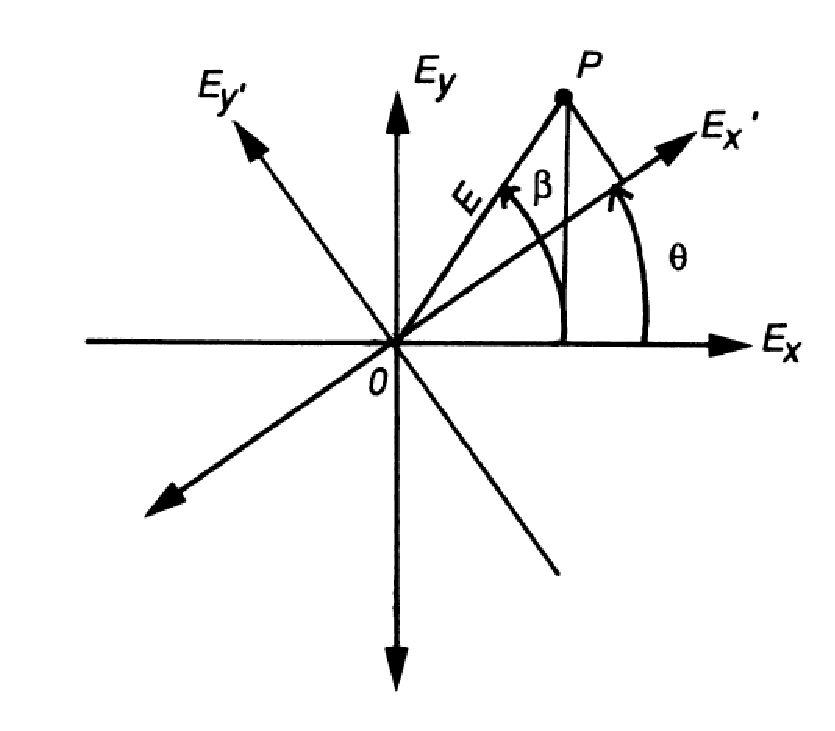
\includegraphics[width = 0.35\textwidth]{Chapter4/Figures/rotator.eps}
 \caption{Rotation of the opticalto Polarization field components by rotator}
 \label{fig:rotator}
\end{figure}
%\vspace{-1cm}

\begin{equation}
	\label{Eq:Rot}
\small
	E'_{x} = E_{x}\cos\theta + E_{y}\sin\theta \hspace{1 cm}
	E'_{y} = -E_{x}\sin\theta + E_{y}\cos\theta~. 
\end{equation}

\begin{equation}
\label{Eq:GenRotMul}
\small
	M(2\theta)= 
	\begin{bmatrix}
	1   & & 0  & & 0  & &0\\ 0   & &\cos 2\theta  & &\sin 2\theta  & &0\\0  & & -\sin 2\theta   & & \cos 2\theta  & & 0\\0  & &0  & & 0  & & 1\\
	\end{bmatrix}~.
\end{equation}

\end{description}
 

The polarizer and retarder are often rotated while being used in optics.
For this reason, it is useful to mention the Mueller matrix of the rotated polarizer and rotated retarder.
First, assume the polarizer is rotated at the same time.
The incident beam first goes through the rotator with the Mueller matrix of $M_{R}(2\theta)$, and then through the polarizer with the Mueller matrix ($M$).
In this case, the emerging Stokes vector in terms of original axis is given by \ref{Eq:rotpol}.
Eq.~\ref{Eq:RotPolMul} represents the Mueller matrix of the rotated polarizer.
%which is the result of multiplying inverse rotation Mueller matrix, the angular form of polarizer Mueller matrix and rotation Mueller matrix. 
\begin{equation}\label{Eq:rotpol}
\small
	S' = M_{R}(-2\theta)MM_{R}(2\theta)~.
\end{equation}

\begin{equation}\label{Eq:RotPolMul}
\small
	M = \frac{p^{2}}{2} 
	\begin{bmatrix}
	 1  & & \cos 2\gamma\cos 2\theta  & & \cos 2\gamma \sin 2\theta  & & 0\\ 
	 \cos 2\gamma\cos 2\theta   & & \cos^{2} 2\theta + \sin 2\gamma \sin^{2} 2\theta  & & (1-\sin 2\gamma)\sin 2\theta \cos 2\theta  & &  0\\
	 \cos 2\gamma \sin 2\theta   & & (1-\sin 2\gamma)\sin 2\theta \cos 2\theta  & & \sin^{2} 2\theta + \sin 2\gamma \cos^{2} 2\theta  & & 0\\
	 0  & & 0  & & 0  & & \sin 2\gamma\\
	\end{bmatrix}~,   
\end{equation}

\noindent The matrix represented in Eq.~\ref{Eq:RotPolMul} is the general form.
Thus, for different values of $\gamma = 0^{\circ} , 45^{\circ}$ and $90^{\circ}$, the matrix represent the linear horizontal polarizer, the neutral density filter and the linear vertical polarizer, respectively.
The Mueller matrix of an ideal linear horizontal polarizer is shown in Eq.~\ref{Eq:HRotPolMul}. 
\begin{equation}\label{Eq:HRotPolMul}
\small
	M = \frac{1}{2} 
	\begin{bmatrix}
	 1  & & \cos 2\theta  & & \sin 2\theta  & & 0\\ 
	 \cos 2\theta   & & \cos^{2} 2\theta  & & \sin 2\theta \cos 2\theta  & & 0\\
	  \sin 2\theta   & & \sin 2\theta \cos 2\theta  & & \sin^{2} 2\theta   & & 0\\
	 0  & &0  & &0  & &0\\
	\end{bmatrix}~.
\end{equation}
%Table \ref{Tab:Chp4T3} represents the Mueller matrices for horizontal, vertical and $\pm 45^{\circ}$ linear and circular polarizers. 
%\begin{table}
\small
\begin{center}
\caption{Mueller matrix of linear horizontal and vertical polarizers and circular polarizer.}
\begin{tabular}{ c c c }
    \hline
    & & \\[-2.5ex]
    H/V & $\pm 45^{\circ}$ & R/L\\
	& & \\[-2.5ex]    
    \hline   
    & & \\[-1.5ex] 
   $\begin{bmatrix}
    1 & & \pm 1 & & 0 & & 0 \\  \pm 1 & & 1 & & 0 & & 0 \\  0 & & 0 & & 0 & & 0 \\  0 & & 0 & & 0 & & 0     
   \end{bmatrix}$ &    
   $\begin{bmatrix}
   1 & & 0 & & \pm 1 & & 0 \\  0 & & 0 & & 0 & & 0 \\  \pm 1 & & 0 & & 1 & & 0 \\  0 & & 0 & & 0 & & 0   
   \end{bmatrix}$& 
   $\begin{bmatrix}
   1 & & 0 & & 0 & & \pm 1 \\  0 & & 0 & & 0 & & 0 \\  0 & & 0 & & 0 & & 0 \\  \pm 1 & & 0 & & 0 & & 1     
   \end{bmatrix}$\\   
    &  &    \\
       \hline   
  \end{tabular}
  \label{Tab:Chp4T3}
  \end{center}
\end{table}

\noindent The Mueller matrix of a rotated retarder is calculated in the same manner.
Equation.~\ref{Eq:RotRetMul} represents the general form of rotated retarder Mueller matrix. 
\begin{equation}\label{Eq:RotRetMul}
\small
	M(\phi , 2\theta)= 
	\begin{bmatrix}
	 1  & & 0  & & 0  & & 0\\ 
	 0  & &\cos^{2} 2\theta + \cos \phi \sin^{2} 2\theta  & & (1-\cos \phi)\sin 2\theta \cos 2\theta  & &   -\sin \phi \cos 2\theta\\
	 0  & & (1-\cos\phi)\sin 2\theta \cos 2\theta  & & \sin^{2} 2\theta + \sin \phi \cos^{2} 2\theta  & & \sin \phi \cos 2\theta\\
	 0  & & \sin \phi \sin 2\theta  & & -\sin \phi \cos 2\theta  & &\cos \phi\\
	\end{bmatrix}~.
\end{equation}

